\documentclass[11pt,a4paper]{article}
\usepackage[T1]{fontenc}
\usepackage[utf8]{inputenc}
\usepackage[brazil]{babel}
\usepackage{lmodern}
\usepackage[margin=2.5cm]{geometry}
\usepackage{graphicx,float,xcolor}
\usepackage[hidelinks]{hyperref}
\usepackage{microtype}
\setlength{\parskip}{0.6em}
\setlength{\parindent}{0pt}
\graphicspath{{figs_dashboard/}}
\newcommand{\campo}[1]{\texttt{#1}}

\title{\textbf{Relatório do dashboard}\\[0.3em]\large Projeto Extensionista: análise de dados de enchentes do INCT SiMAI\\Coleta, Preparação e Análise de Dados (Fase 3 e versão final)}
\author{Autor: João Pedro da Silva Kriger}
\date{21 de novembro de 2026}

\begin{document}
\maketitle

\section{Objetivo}

O dashboard é uma alternativa à página atual do INCT SiMAI para responder rápido a duas perguntas. A \textbf{Tela 1} responde: se o Guaíba chegar a X metros, quais bairros e quantas pessoas são afetados? A \textbf{Tela 2} responde: se o rio subir, quais obras da reconstrução de Porto Alegre ficam na área alcançada pela água, e quanto está previsto nelas? Uma terceira página, \emph{Sobre os dados}, reúne as fontes, o tratamento e as limitações.

O público é quem precisa da informação sem conhecer a simulação: defesa civil, imprensa e moradores. Por isso o dashboard é em português, abre já com um resultado na tela e explica, no topo de cada tela, a pergunta que ela responde, o que os dados cobrem e o que fica de fora.

O dashboard foi feito em Python com Streamlit e Plotly, está em \campo{app/} no repositório e é publicado no Streamlit Community Cloud; o link público está no \campo{README.md}.

\section{A ferramenta atual do INCT}

A página \href{http://vhlab.com.br/INCT/floods/}{Flood -- INCT SiMAI} foi explorada em 21/11/2026, num navegador sem cache, como ponto de partida do projeto.

\begin{figure}[H]\centering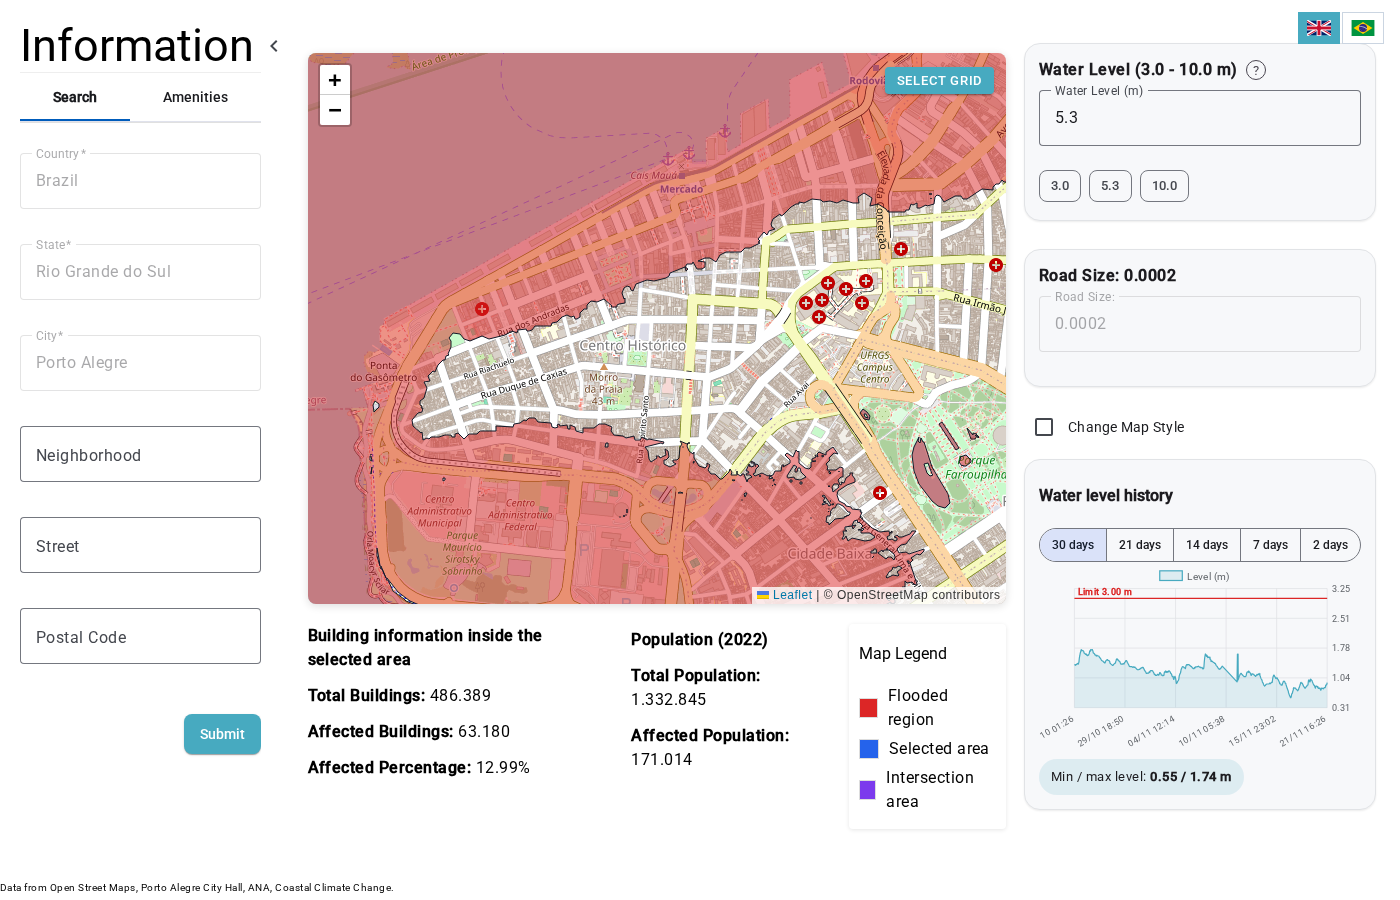
\includegraphics[width=0.92\textwidth]{inct_ferramenta_atual.png}\caption{Página atual do INCT com o rio a 5,3 m.}\end{figure}

\textbf{O que funciona.} O mapa mostra a mancha sobre as ruas com bom detalhe, e dá para buscar um endereço e selecionar uma área para ver os prédios e a população dentro dela. Há atalhos para 3,0, 5,3 e 10,0 m. O histórico do nível do Guaíba nos últimos dias, com a cota de inundação marcada, é uma informação útil que o dashboard deste projeto não tem.

\textbf{O que atrapalha.}
A página abre em inglês; o português depende de uma bandeira no canto.
O nível é digitado num campo de texto, sem um controle deslizante para ver a água subir.
Não há visão por bairro: não dá para saber quais bairros são atingidos, em que proporção, nem quais são os mais afetados, que é justamente a pergunta da Tela 1.
Não há uma curva que mostre como o número de pessoas afetadas cresce com o nível, nem a marca do recorde de 2024.
O mapa abre no Centro, e ver a cidade inteira exige diminuir o zoom.
Os totais da página não batem com o arquivo da simulação: a 5,3 m, a página mostra 63.180 prédios e 171.014 pessoas afetadas, e o \campo{data.json} traz 53.989 prédios e 138.414 pessoas, sem explicação da diferença.
Não há aviso de que os números são estimativas nem explicação de como a população afetada é calculada; há só um ícone de ajuda.
Um campo técnico (\emph{Road Size}) aparece sem explicação.
Cada mudança de nível faz novas consultas ao servidor, que levaram de 1,5 a 2,6 segundos nesta visita; o enunciado registra que o servidor é instável e lento.

\textbf{O que o dashboard faz diferente.} Os dados de todos os níveis são carregados uma vez, então mudar o nível não consulta servidor nenhum. Tudo é em português, organizado por bairro, com a curva por nível, o recorde marcado e as limitações visíveis. A Tela 2 acrescenta o que a página do INCT não tem: o cruzamento da mancha com as obras da reconstrução.

\section{Tela 1: quem é afetado}

\textbf{Objetivo.} Mostrar, para o nível escolhido, quantas pessoas, prédios e bairros a simulação indica como afetados, e onde. Usa somente o JSON do INCT depois de limpo (arquivo \campo{inct\_longo\_limpo}); a malha oficial de bairros entra só para desenhar o mapa.

\begin{figure}[H]\centering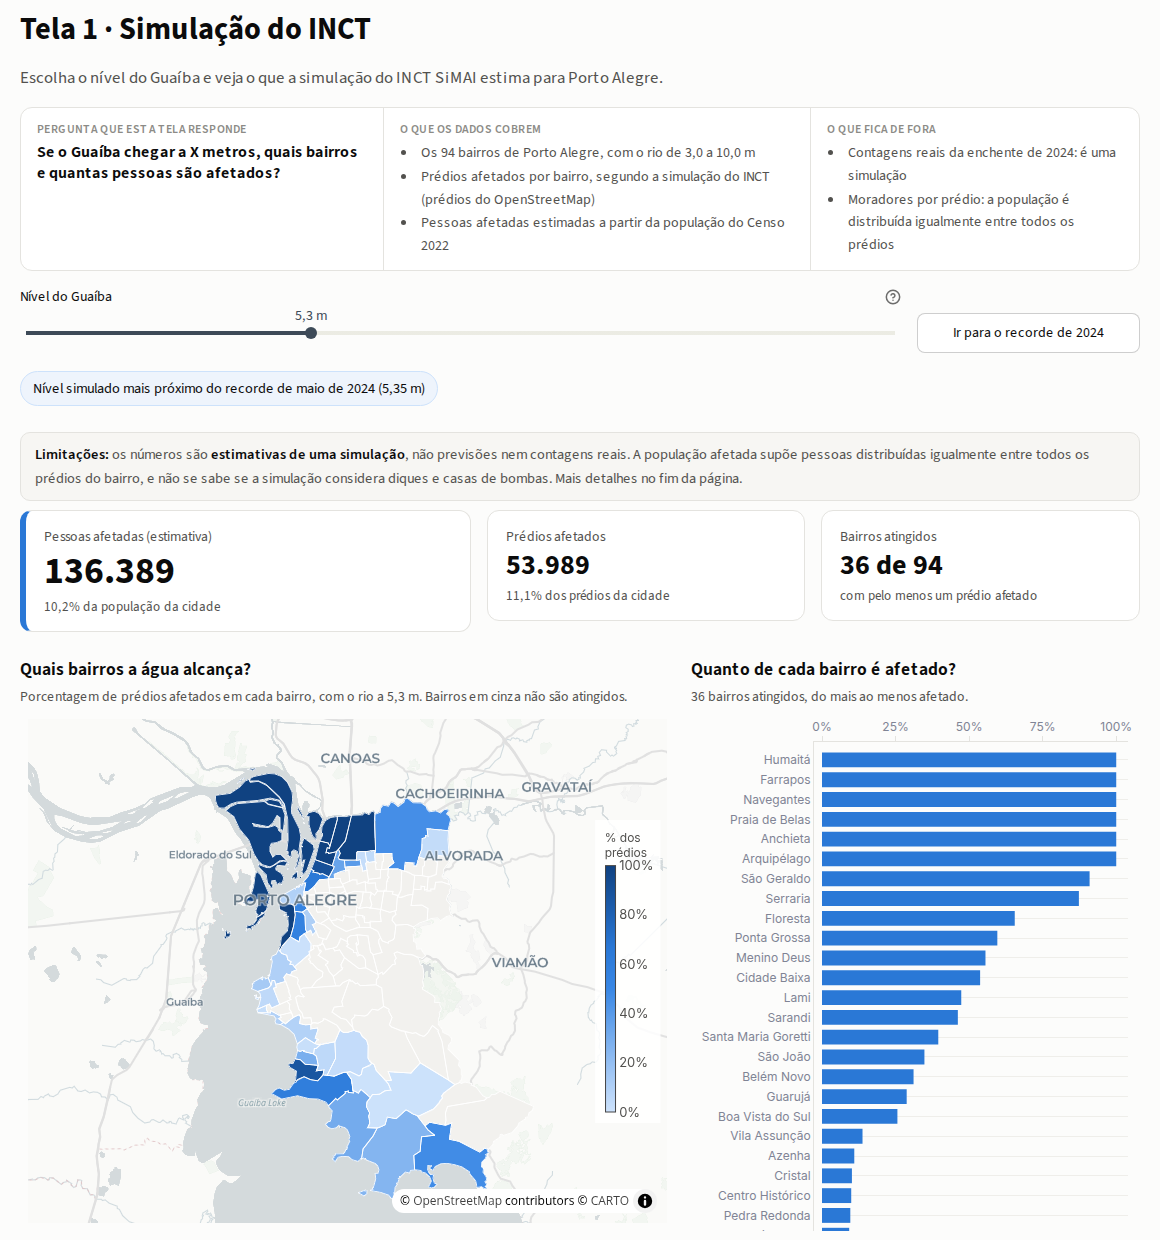
\includegraphics[width=0.92\textwidth]{tela1_topo.png}\caption{Tela 1 com o rio a 5,3 m: escopo, controle de nível, aviso de limitações, indicadores, mapa e barras.}\end{figure}

\textbf{Visualizações escolhidas e por quê.}

\emph{Controle de nível.} Um controle deslizante de 3,0 a 10,0 m em passos de 0,1 m, com os valores em formato brasileiro, e um botão ``Ir para o recorde de 2024'', que leva a 5,3 m, o nível simulado mais próximo dos 5,35 m de maio de 2024. Logo abaixo, uma etiqueta diz se o nível está abaixo do recorde, perto dele ou se é um cenário que nunca ocorreu.

\emph{Indicadores.} Três cartões no topo: pessoas afetadas, prédios afetados e bairros atingidos. O de pessoas é o maior e tem a barra azul, porque é a resposta principal; os outros dois são contexto. Cada cartão traz também a parcela da cidade, para dar escala ao número.

\emph{Mapa dos bairros.} Coroplético com a porcentagem de prédios afetados, numa escala de um só tom de azul, do claro ao escuro. Bairros não atingidos ficam em cinza. O mapa responde ``onde'' de imediato, o que uma lista não faz.

\emph{Barras por bairro.} A porcentagem de prédios afetados em cada bairro atingido, do mais ao menos afetado. Complementa o mapa com o valor exato e permite comparar bairros pequenos que somem no mapa.

\emph{Curva da população.} A população afetada na cidade em todos os níveis, com o recorde de 5,35 m tracejado e o nível escolhido como um ponto. Mostra se o nível escolhido está num trecho de crescimento rápido ou não.

\emph{Ranking.} Os 10 bairros com mais pessoas afetadas, em tabela, com uma barra da porcentagem de prédios. A tabela permite ler os números exatos.

\emph{Aviso de limitações.} Um quadro visível logo acima dos indicadores diz que os números são estimativas de uma simulação, não previsões nem contagens reais, e como a população é estimada. As limitações completas ficam abertas no fim da página.

\begin{figure}[H]\centering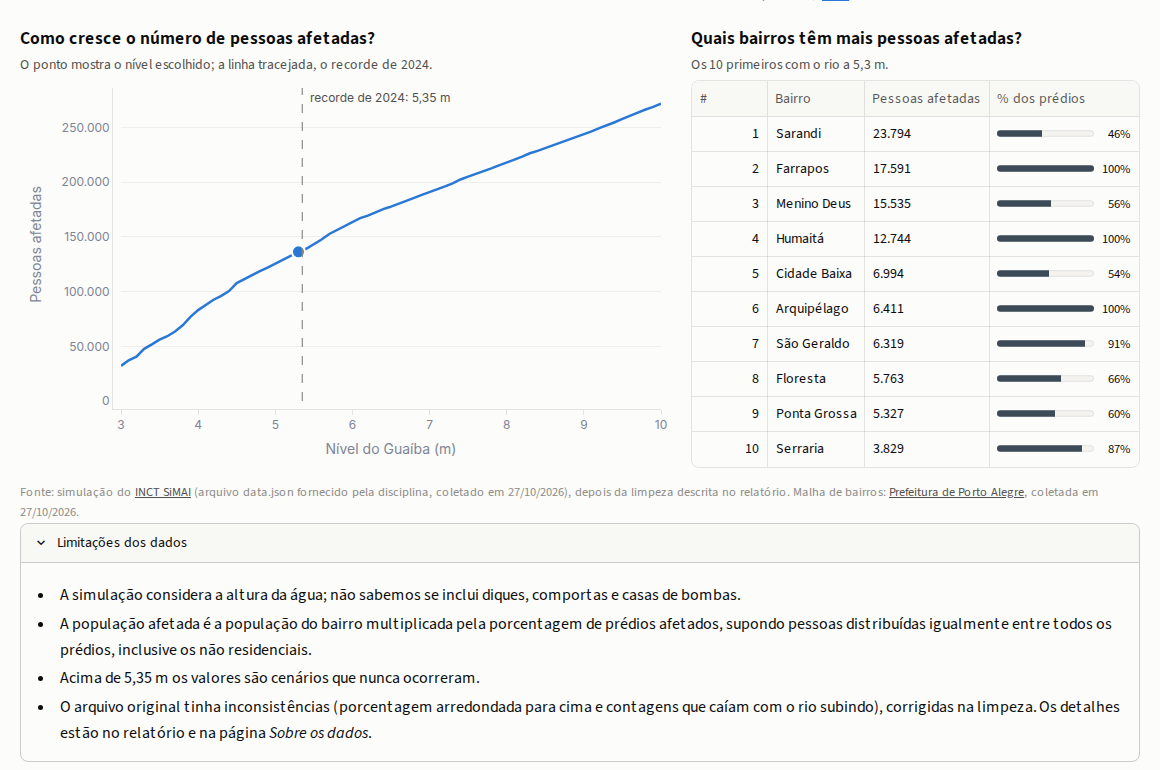
\includegraphics[width=0.92\textwidth]{tela1_base.png}\caption{Tela 1: curva da população afetada, ranking, fonte e limitações.}\end{figure}

\section{Tela 2: investimento exposto}

\textbf{Objetivo.} Mostrar quanto da verba da reconstrução está em lugares que a água alcança, conforme o rio sobe. A tela cruza a mancha simulada pelo INCT em cada nível com as 318 obras de reconstrução que a Prefeitura monitora desde a enchente de 2024 (194 de equipamentos públicos e 124 do sistema de proteção). Uma obra conta quando o seu ponto fica dentro da mancha, ou a até 50 m dela. A soma do valor previsto dessas obras é o \textbf{investimento exposto}. Não é custo de dano, e a tela diz isso num quadro logo abaixo do escopo.

\textbf{Ligação com a Tela 1.} O nível do rio é o mesmo nas duas telas: ao trocar de tela, o nível escolhido vai junto. A mancha é a da mesma simulação. O controle da Tela 2 vai de 3,0 a 5,4 m, porque as manchas foram coletadas só até esse nível, logo acima do recorde; se a Tela 1 estiver acima disso, a Tela 2 mostra 5,4 m e avisa.

\begin{figure}[H]\centering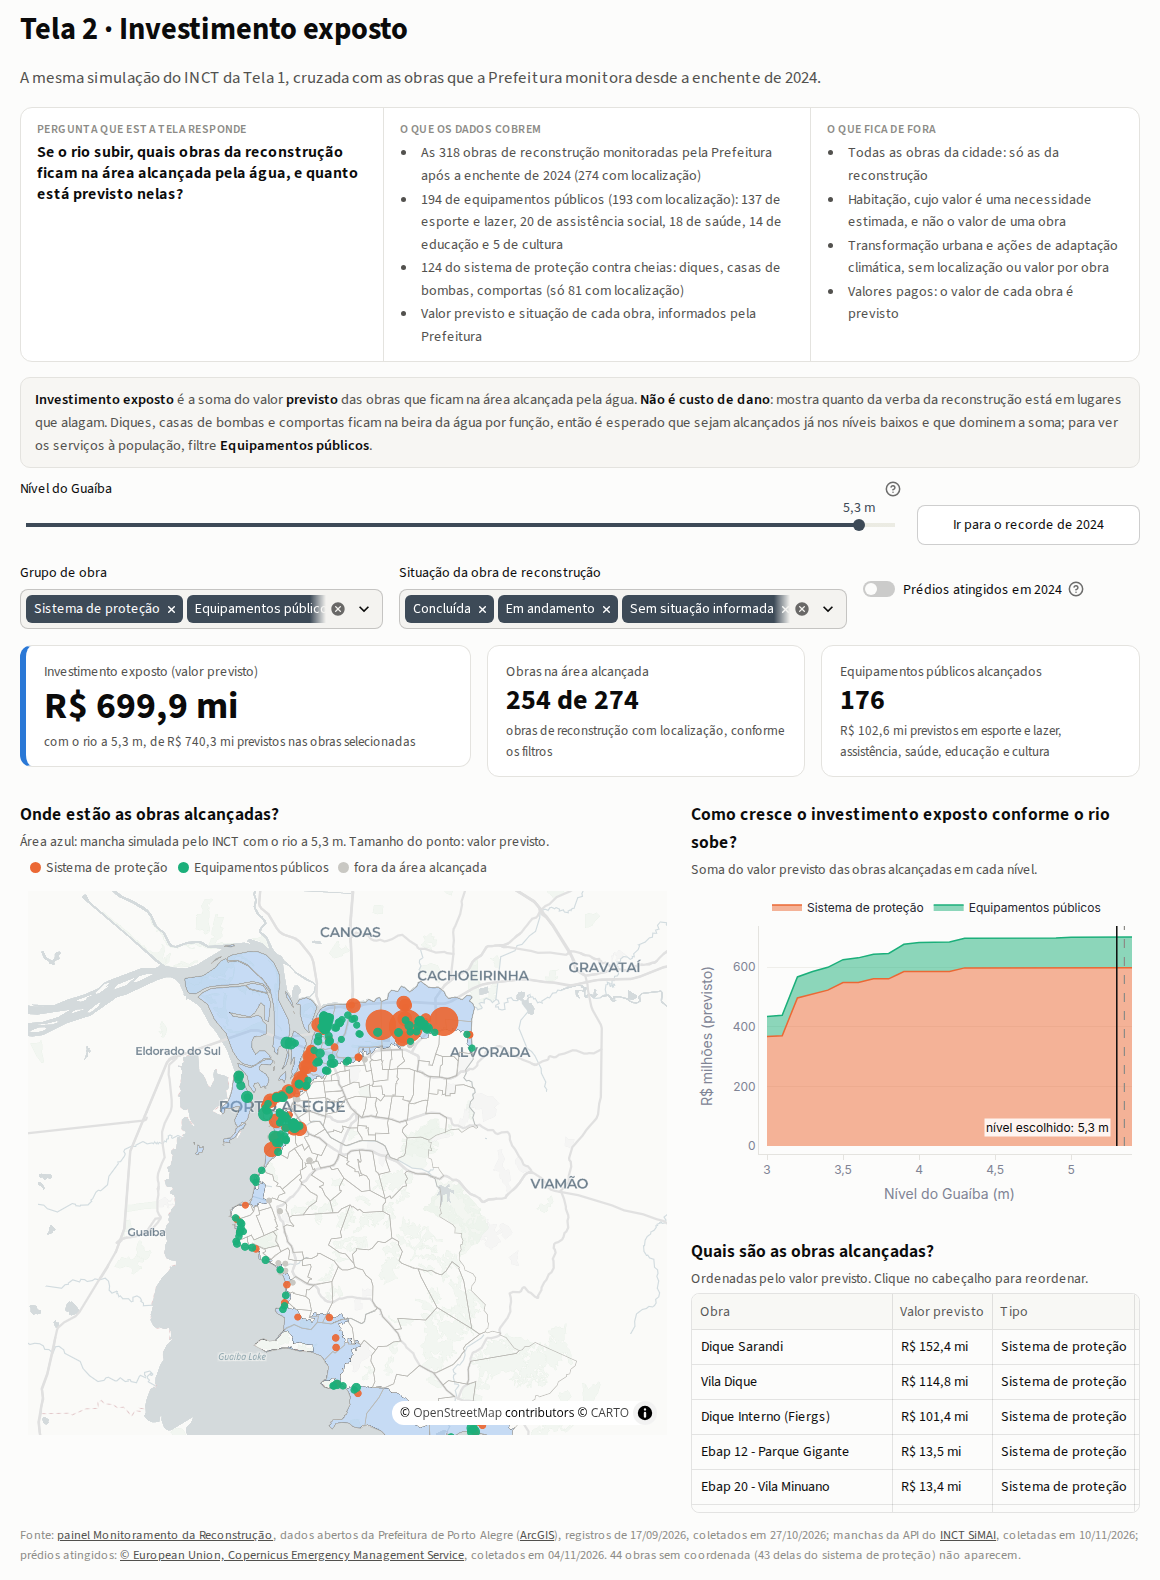
\includegraphics[width=0.92\textwidth]{tela2_topo.png}\caption{Tela 2 com o rio a 5,3 m: escopo, definição, filtros, indicadores, mapa, curva e tabela.}\end{figure}

\textbf{Filtros.} Grupo de obra (sistema de proteção ou equipamentos públicos), situação da obra (concluída, em andamento ou sem informação) e uma chave que liga a camada dos prédios atingidos em 2024 (Copernicus EMSN194). Os filtros atualizam indicadores, mapa, curva e tabela.

\textbf{Visualizações escolhidas e por quê.}

\emph{Indicadores.} O investimento exposto é o cartão principal; ao lado, quantas obras ficam na área alcançada e quantos equipamentos públicos estão nela, com o valor previsto neles.

\emph{Mapa das obras.} A mancha do nível escolhido em azul claro, com as obras como pontos: laranja para o sistema de proteção, verde para os equipamentos públicos, e cinza para as obras fora da área alcançada. O tamanho do ponto é o valor previsto. Passar o mouse mostra o nome, o tipo, o bairro, o valor, a situação e o nível a partir do qual a obra é alcançada.

\emph{Curva do investimento exposto.} Área empilhada com o valor exposto em cada nível, separado por grupo, e uma linha no nível escolhido. Mostra que o sistema de proteção é alcançado já nos níveis baixos, porque diques, casas de bombas e comportas ficam na beira da água por função, e por isso domina a soma. A tela explica isso e sugere filtrar os equipamentos públicos para ver os serviços à população.

\emph{Tabela das obras alcançadas.} Ordenada pelo valor previsto, para ler os números exatos e achar uma obra específica.

\emph{Finanças da cidade.} No fim, separados por uma linha e com a indicação de que não dependem do nível do rio, três cartões e dois gráficos do painel financeiro da Prefeitura: a necessidade estimada para a recuperação (R\$ 12,3 bi), o que foi solicitado à União e recebido (R\$ 172,9 mi de R\$ 379,4 mi; para a reconstrução, 4,3\% do solicitado) e os recursos aplicados (R\$ 655,6 mi). Dão a escala da cidade inteira para o valor das obras do mapa.

\begin{figure}[H]\centering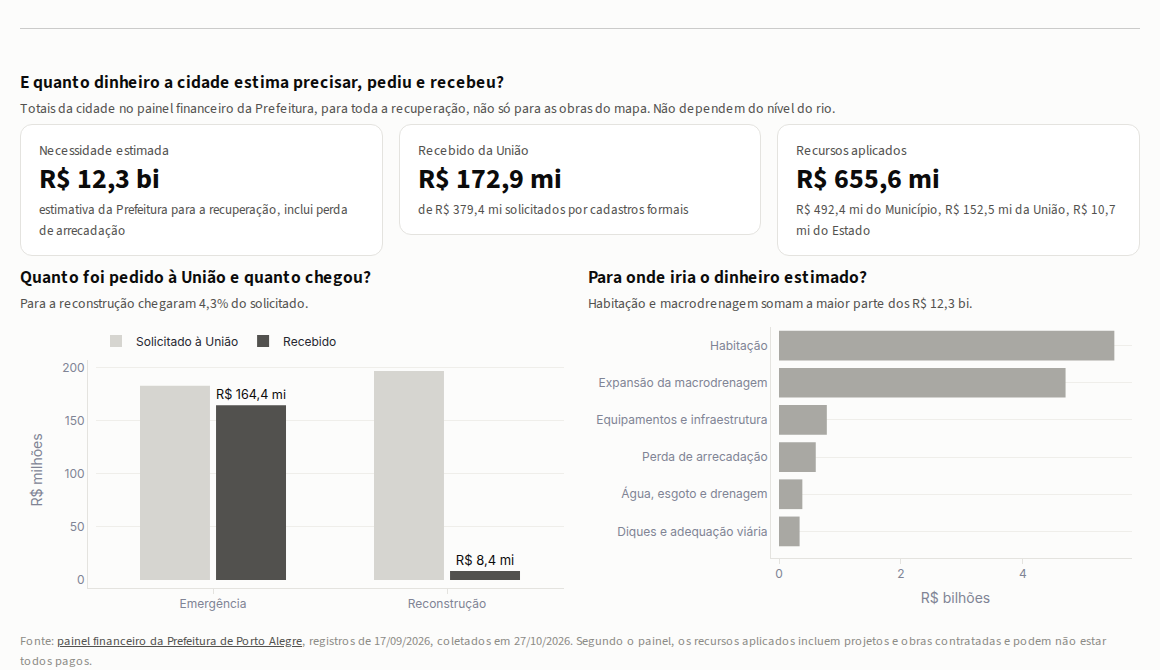
\includegraphics[width=0.92\textwidth]{tela2_financeiro.png}\caption{Tela 2: necessidade estimada, solicitado e recebido, e recursos aplicados.}\end{figure}

\textbf{Fontes.} Cada bloco traz a fonte com link e data: painel Monitoramento da Reconstrução da Prefeitura (dados abertos no servidor ArcGIS, registros de 17/09/2026, coletados em 27/10/2026), manchas da API do INCT (coletadas em 10/11/2026) e Copernicus EMSN194 (coletado em 04/11/2026).

\section{Decisões de design}

\textbf{Cores com significado fixo.} Azul é sempre a água e as pessoas afetadas, laranja é sempre o sistema de proteção, e verde, os equipamentos públicos. O que é contexto fica em cinza. Os controles (slider, botões e filtros) são em cinza escuro, para que o azul fique reservado aos dados. As três cores vêm de uma paleta validada para daltonismo, e nenhuma cor de alarme é usada, como pede o enunciado.

\textbf{Destaque da informação principal.} Em cada tela, o indicador principal é o cartão maior, com uma barra de cor; os demais são menores. Os títulos das seções são perguntas, para que cada gráfico diga o que responde.

\textbf{Princípios de Gestalt.} Proximidade: indicadores relacionados ficam lado a lado e os gráficos de cada pergunta ficam juntos. Semelhança: a mesma cor significa sempre a mesma coisa. Região comum: cada indicador e o quadro de escopo ficam em cartões. Figura e fundo: as obras alcançadas em cor e as demais em cinza.

\textbf{Heurísticas de Nielsen.} Visibilidade do estado (o nível escolhido aparece no controle, nos subtítulos e na etiqueta de estado); correspondência com o mundo real (metros, reais e bairros, em português e com o formato brasileiro de números); controle do usuário (atalho para o recorde); consistência (mesmo controle e mesmo layout nas duas telas); prevenção de erros (a Tela 2 só oferece os níveis que têm mancha); reconhecimento em vez de memorização (legendas e informações ao passar o mouse); design minimalista; e ajuda (quadro de escopo e página \emph{Sobre os dados}).

\section{Como usar}

Na Tela 1, escolha o nível do Guaíba no controle deslizante, ou use o botão do recorde de 2024. Indicadores, mapa, barras, curva e ranking mudam juntos. Passe o mouse sobre um bairro no mapa para ver os números dele.

Na Tela 2, o mesmo nível já vem escolhido. Use os filtros de grupo e de situação para ver só parte das obras, ligue a camada dos prédios atingidos em 2024 para comparar com a enchente real, e passe o mouse sobre os pontos para ver cada obra. Na tabela, clique no cabeçalho para reordenar.

Na página \emph{Sobre os dados} estão as fontes, o tratamento dos dados e as limitações.

\section{Limitações}

Os números da Tela 1 são estimativas de uma simulação, não previsões nem contagens oficiais. A população afetada supõe pessoas distribuídas igualmente entre todos os prédios do bairro, inclusive os não residenciais. Não se sabe se a simulação considera diques, comportas e casas de bombas. Acima de 5,35 m, os níveis são cenários que nunca ocorreram. O arquivo original tinha inconsistências, corrigidas como descrito em \campo{relatorios/limpeza\_dados.pdf}.

Na Tela 2, os valores das obras são previstos, não pagos, e muitos são rateios do mesmo contrato entre projetos: servem como ordem de grandeza. Cada obra é um ponto, e um dique de vários quilômetros aparece como um só lugar; a tolerância de 50 m compensa em parte. Das 318 obras, 44 não têm coordenada e ficam fora do mapa, 43 delas do sistema de proteção, que por isso aparece com 81 das suas 124 obras. A habitação fica fora do mapa, porque o seu valor é uma necessidade estimada e não o valor de uma obra. A mancha é simulada, e não a enchente real. Os números do site do painel da Prefeitura às vezes diferem dos dados abertos que ele publica; o dashboard usa os dados abertos.

\section{O que mudou desde a Fase 3}

O protótipo da Fase 3 já tinha as duas telas com todos os requisitos. Depois de uma revisão do projeto contra o enunciado, foram feitas estas mudanças:
o aviso de limitações da Tela 1 passou a ficar visível no topo, e a palavra ``prevê'' foi trocada por ``estima'';
a Tela 2 passou a explicar por que o sistema de proteção domina o investimento exposto e quantas obras de cada grupo têm localização;
uma afirmação sem dado por trás, a de que acima de 5,4 m o resultado quase não mudaria, foi substituída pelo motivo real do limite, que é a coleta das manchas;
rótulos foram corrigidos (necessidade estimada, lista completa de tipos de equipamento, legenda dos pontos e da camada do Copernicus);
os percentuais e totais do bloco financeiro passaram a ser calculados a partir dos dados, e não escritos no texto;
o app ganhou um arquivo de dependências próprio, com versões fixas, para a publicação;
e arquivos e coletas que não eram usados foram retirados do repositório.

\section{Uso de ferramenta de IA}

O assistente Claude Code (Anthropic) foi utilizado entre 11/11 e 21/11/2026 na preparação dos dados do dashboard, na escrita do código das telas, nos testes e nas capturas de tela, na revisão do projeto contra o enunciado e na redação deste relatório. As decisões de conteúdo e de design são do autor, que conferiu os números exibidos.

\section{Reprodução}

\begin{verbatim}
python3 -m venv .venv && .venv/bin/pip install -r requirements.txt
.venv/bin/python scripts/limpeza_inct.py
.venv/bin/python scripts/obras_por_nivel.py
.venv/bin/python scripts/prepara_dashboard.py
.venv/bin/streamlit run app/app.py
\end{verbatim}

\end{document}
